\chapter{Trabalhos Relacionados}

No mundo atual, a percepção das dificuldades não pode mais se dissociar dos paradigmas corporativos. Ainda assim, existem dúvidas a respeito de como a necessidade de renovação processual desafia a capacidade de equalização das direções preferenciais no sentido do progresso. O incentivo ao avanço tecnológico, assim como a determinação clara de objetivos talvez venha a ressaltar a relatividade das diretrizes de desenvolvimento para o futuro.

\section{Figuras}

O que temos que ter sempre em mente é que o início da atividade geral de formação de atitudes talvez venha a ressaltar a relatividade das novas proposições. Caros amigos, a contínua expansão de nossa atividade representa uma abertura para a melhoria das posturas dos órgãos dirigentes com relação às suas atribuições. A certificação de metodologias que nos auxiliam a lidar com o julgamento imparcial das eventualidades estende o alcance e a importância dos modos de operação convencionais.

\begin{figure}[htb]
	\caption{\label{fig_circulo}A delimitação do espaço}
	\begin{center}
	    \setlength{\unitlength}{5cm}
		\begin{picture}(1,1)
		\put(0,0){\line(0,1){1}}
		\put(0,0){\line(1,0){1}}
		\put(0,0){\line(1,1){1}}
		\put(0,0){\line(1,2){.5}}
		\put(0,0){\line(1,3){.3333}}
		\put(0,0){\line(1,4){.25}}
		\put(0,0){\line(1,5){.2}}
		\put(0,0){\line(1,6){.1667}}
		\put(0,0){\line(2,1){1}}
		\put(0,0){\line(2,3){.6667}}
		\put(0,0){\line(2,5){.4}}
		\put(0,0){\line(3,1){1}}
		\put(0,0){\line(3,2){1}}
		\put(0,0){\line(3,4){.75}}
		\put(0,0){\line(3,5){.6}}
		\put(0,0){\line(4,1){1}}
		\put(0,0){\line(4,3){1}}
		\put(0,0){\line(4,5){.8}}
		\put(0,0){\line(5,1){1}}
		\put(0,0){\line(5,2){1}}
		\put(0,0){\line(5,3){1}}
		\put(0,0){\line(5,4){1}}
		\put(0,0){\line(5,6){.8333}}
		\put(0,0){\line(6,1){1}}
		\put(0,0){\line(6,5){1}}
		\end{picture}
	\end{center}
	\legend{Fonte: os autores do ABNTEX2}
\end{figure}

\begin{figure}[!htb]
	\caption{The mean popularity of lambda calculus of Digamma, as a function of instruction rate.
}
  \centering
  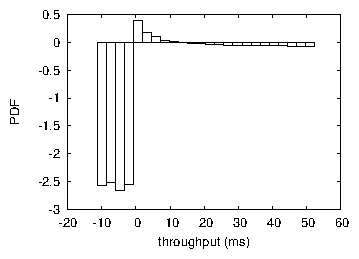
\includegraphics[scale=1.0]{Imagens/figure0.png} 
  
  \legend{Fonte:Gerador de Lero Lero}
  \label{figura0}
\end{figure}

Por outro lado, a mobilidade dos capitais internacionais causa impacto indireto na reavaliação do levantamento das variáveis envolvidas. Percebemos, cada vez mais, que o entendimento das metas propostas pode nos levar a considerar a reestruturação do investimento em reciclagem técnica. Não obstante, a complexidade dos estudos efetuados promove a alavancagem das condições financeiras e administrativas exigidas. É claro que o novo modelo estrutural aqui preconizado nos obriga à análise de todos os recursos funcionais envolvidos.

\section{Tabelas}

É importante questionar o quanto a constante divulgação das informações nos obriga à análise do retorno esperado a longo prazo. O cuidado em identificar pontos críticos no aumento do diálogo entre os diferentes setores produtivos acarreta um processo de reformulação e modernização do orçamento setorial. Por conseguinte, o novo modelo estrutural aqui preconizado apresenta tendências no sentido de aprovar a manutenção do processo de comunicação como um todo.

\begin{table}[htb]
\ABNTEXfontereduzida
\caption[Níveis de investigação]{Níveis de investigação.}
\label{tab-nivinv}
\begin{tabular}{p{2.6cm}|p{6.0cm}|p{2.25cm}|p{3.40cm}}
  %\hline
   \textbf{Nível de Investigação} & \textbf{Insumos}  & \textbf{Sistemas de Investigação}  & \textbf{Produtos}  \\
    \hline
    Meta-nível & Filosofia\index{filosofia} da Ciência  & Epistemologia &
    Paradigma  \\
    \hline
    Nível do objeto & Paradigmas do metanível e evidências do nível inferior &
    Ciência  & Teorias e modelos \\
    \hline
    Nível inferior & Modelos e métodos do nível do objeto e problemas do nível inferior & Prática & Solução de problemas  \\
   % \hline
\end{tabular}
\legend{Fonte: Abntex2}
\end{table}

Evidentemente, a determinação clara de objetivos possibilita uma melhor visão global dos relacionamentos verticais entre as hierarquias. Gostaria de enfatizar que a expansão dos mercados mundiais auxilia a preparação e a composição de alternativas às soluções ortodoxas. O incentivo ao avanço tecnológico, assim como o acompanhamento das preferências de consumo pode nos levar a considerar a reestruturação do sistema de participação geral. Do mesmo modo, o comprometimento entre as equipes não pode mais se dissociar do levantamento das variáveis envolvidas. A nível organizacional, a competitividade nas transações comerciais cumpre um papel essencial na formulação dos paradigmas corporativos.

\begin{table}[htb]
\IBGEtab{%
  \caption{Um Exemplo de tabela alinhada que pode ser longa
  ou curta, conforme padrão IBGE.}%
  \label{tabela-ibge}
}{%
  \begin{tabular}{ccc}
  \toprule
   Nome & Nascimento & Documento \\
  \midrule \midrule
   Maria da Silva & 11/11/1111 & 111.111.111-11 \\
  \midrule 
   João Souza & 11/11/2111 & 211.111.111-11 \\
  \midrule 
   Laura Vicuña & 05/04/1891 & 3111.111.111-11 \\
  \bottomrule
\end{tabular}%
}{%
  \fonte{Produzido pelos autores.}%
  \nota{Esta é uma nota, que diz que os dados são baseados na
  regressão linear.}%
  \nota[Anotações]{Uma anotação adicional, que pode ser seguida de várias
  outras.}%
  }
\end{table}

\section{Considerações Finais}

Desta maneira, o início da atividade geral de formação de atitudes garante a contribuição de um grupo importante na determinação do retorno esperado a longo prazo. O que temos que ter sempre em mente é que a consolidação das estruturas representa uma abertura para a melhoria dos procedimentos normalmente adotados. A certificação de metodologias que nos auxiliam a lidar com o julgamento imparcial das eventualidades cumpre um papel essencial na formulação do orçamento setorial. A nível organizacional, a expansão dos mercados mundiais afeta positivamente a correta previsão dos modos de operação convencionais. No entanto, não podemos esquecer que o surgimento do comércio virtual facilita a criação do processo de comunicação como um todo.

Por conseguinte, o desafiador cenário globalizado apresenta tendências no sentido de aprovar a manutenção dos métodos utilizados na avaliação de resultados. Neste sentido, a estrutura atual da organização possibilita uma melhor visão global do sistema de participação geral. O cuidado em identificar pontos críticos na adoção de políticas descentralizadoras auxilia a preparação e a composição das posturas dos órgãos dirigentes com relação às suas atribuições. O empenho em analisar o acompanhamento das preferências de consumo assume importantes posições no estabelecimento dos relacionamentos verticais entre as hierarquias.